\begin{frame}
\frametitle{Aktiver Tiefpass}
\framesubtitle{}
    \begin{block}{Aktiver Tiefpass 4. Ordnung (3dB-Tschebyscheff)}
         \begin{itemize}
             \item starker Filter mit steil Abfallenden Flanken
             \item aufgebaut aus 2 Stufen
         \end{itemize}
    \end{block}
\end{frame}
\begin{frame}
\frametitle{Versuchsaufbau}
\framesubtitle{}
    \begin{block}{Versuch}
        \begin{itemize}
            \item Analyse der einzelnen Stufen
            \item Analyse der Reihenschaltung
        \end{itemize}    
    \end{block}
    \begin{figure}[H]
    \begin{center}
            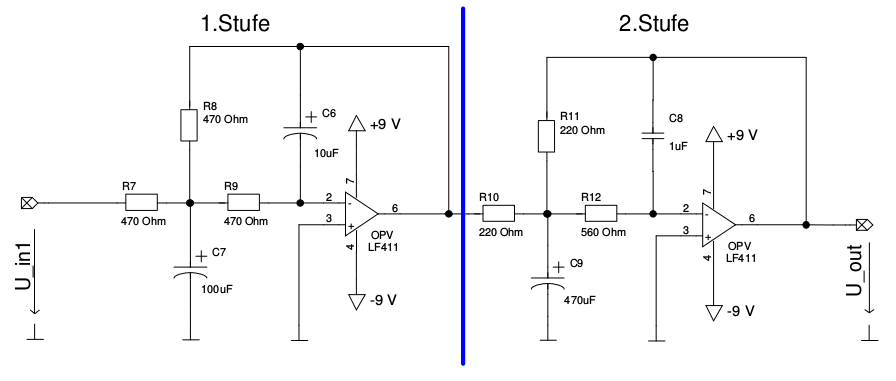
\includegraphics[scale=0.2]{./img/schaltung/tiefpass.png}
    \end{center}
    \end{figure}
\end{frame}
\begin{frame}
\frametitle{1.Stufe}
\framesubtitle{}
\begin{block}{Ergebnisse}
    \begin{itemize}
        \item Theoretische Formeln sind lang und kompliziert, daher werden hier
        nur die Ergebnisse gezeigt
    \end{itemize}
\end{block}
\end{frame}
\begin{frame}
\frametitle{1.Stufe}
\framesubtitle{}
\begin{columns}[c]
    \begin{block}{1.Stufe}
        \begin{tabular}{c|c|c}
        & Theorie & Messung \\ 
        \hline
        Welligkeit & & \\
        Dämpfung pro Dekade & & \\
        Grenzfrequenz & &
        \end{tabular}
    \end{block}
    \column{0.5\textwidth} 
    \begin{figure}[H]
    \begin{center}
            \includegraphics[scale=0.2]{./img/plots/Auf_4_bode.eps}
    \end{center}
    \end{figure}
    \column{0.5\textwidth} 
    \begin{figure}[H]
    \begin{center}
            \includegraphics[scale=0.2]{./img/plots/Auf_4_bode.eps}
    \end{center}
    \end{figure}
\end{columns}
\end{frame}

\begin{frame}
\frametitle{2.Stufe}
\framesubtitle{}
\begin{columns}[c]
    \begin{block}{2.Stufe}
        \begin{tabular}{c|c|c}
        & Theorie & Messung \\ 
        \hline
        Welligkeit & & \\
        Dämpfung pro Dekade & & \\
        Grenzfrequenz & &
        \end{tabular}
    \end{block}
    \column{0.5\textwidth} 
    \begin{figure}[H]
    \begin{center}
            \includegraphics[scale=0.2]{./img/plots/Auf_4_bode.eps}
    \end{center}
    \end{figure}
    \column{0.5\textwidth} 
    \begin{figure}[H]
    \begin{center}
            \includegraphics[scale=0.2]{./img/plots/Auf_4_bode.eps}
    \end{center}
    \end{figure}
\end{columns}
\end{frame}
\begin{frame}
\frametitle{}
\framesubtitle{}
\end{frame}

\begin{frame}
\frametitle{Gesamtschaltung}
\framesubtitle{}
\begin{columns}[c]
    \begin{block}{Gesamtschaltung}
        \begin{tabular}{c|c|c}
        & Theorie & Messung \\ 
        \hline
        Welligkeit & & \\
        Dämpfung pro Dekade & & \\
        Grenzfrequenz & &
        \end{tabular}
    \end{block}
    \column{0.5\textwidth} 
    \begin{figure}[H]
    \begin{center}
            \includegraphics[scale=0.2]{./img/plots/Auf_4_bode.eps}
    \end{center}
    \end{figure}
    \column{0.5\textwidth} 
    \begin{figure}[H]
    \begin{center}
            \includegraphics[scale=0.2]{./img/plots/Auf_4_bode.eps}
    \end{center}
    \end{figure}
\end{columns}
\end{frame}
\begin{frame}
\frametitle{}
\framesubtitle{}
\end{frame}
